\documentclass[10pt]{beamer}
\usepackage[framemethod=TikZ]{mdframed}
\usepackage{pgfpages}
%\setbeameroption{show notes on second screen}
\setbeameroption{show notes}

\usetheme[sectionpage=simple,subsectionpage=simple]{metropolis}
\usepackage{appendixnumberbeamer}

\usepackage{booktabs}
\usepackage[scale=2]{ccicons}

\usepackage{pgfplots}
\usepgfplotslibrary{dateplot}

\usepackage{xspace}
\newcommand{\themename}{\textbf{\textsc{metropolis}}\xspace}

\include{asset/global_usepackage}
\include{asset/global_newcommand}
\include{asset/global_newtheorem}
% %%%%%%%%%%%%%%%%%%%%%%%%%%%%%% 
% % Theorem
% \newcounter{theo}[section] \setcounter{theo}{0}
% \renewcommand{\thetheo}{\arabic{section}.\arabic{theo}}
% \newenvironment{theo}[2][]{%
%   \refstepcounter{theo}%
%   \ifstrempty{#1}%
%   {\mdfsetup{%
%       frametitle={%
%         \tikz[baseline=(current bounding box.east),outer sep=0pt]
%         \node[anchor=east,rectangle,fill=blue!20]
%         {\strut Theorem~\thetheo};}}
%   }%
%   {\mdfsetup{%
%       frametitle={%
%         \tikz[baseline=(current bounding box.east),outer sep=0pt]
%         \node[anchor=east,rectangle,fill=blue!20]
%         {\strut Theorem~\thetheo:~#1};}}%
%   }%
%   \mdfsetup{innertopmargin=-8pt,linecolor=blue!20,%
%     linewidth=2pt,topline=true,%
%     frametitleaboveskip=\dimexpr-\ht\strutbox\relax
%   }
%   \begin{mdframed}[]\relax%
%     \label{#2}}{\end{mdframed}}

%%%%%%%%%%%%%%%%%%%%%%%%%%%%%% 
% Question
\newcounter{question}[section] \setcounter{question}{0}
\renewcommand{\thequestion}{}%{\arabic{section}.\arabic{question}}
\newenvironment{question}[2][]{%
  \refstepcounter{question}%
  \ifstrempty{#1}%
  {\mdfsetup{%
      frametitle={%
        \tikz[baseline=(current bounding box.east),outer sep=0pt]
        \node[anchor=east,rectangle,fill=blue!20]
        {\strut 问题~\thequestion};}}
  }%
  {\mdfsetup{%
      frametitle={%
        \tikz[baseline=(current bounding box.east),outer sep=0pt]
        \node[anchor=east,rectangle,fill=blue!20]
        {\strut 问题~\thequestion:~#1};}}%
  }%
  \mdfsetup{innertopmargin=-8pt,linecolor=blue!20,%
    linewidth=2pt,topline=true,%
    frametitleaboveskip=\dimexpr-\ht\strutbox\relax
  }
  \begin{mdframed}[]\relax%
    \label{#2}}{\end{mdframed}}


% %%%%%%%%%%%%%%%%%%%%%%%%%%%%%% 
% % Property
% \newcounter{prop}[section] \setcounter{prop}{0}
% \renewcommand{\theprop}{}%\arabic{section}.\arabic{prop}}
% \newenvironment{prop}[2][]{%
%   \refstepcounter{prop}%
%   \ifstrempty{#1}%
%   {\mdfsetup{%
%       frametitle={%
%         \tikz[baseline=(current bounding box.east),outer sep=0pt]
%         \node[anchor=east,rectangle,fill=green!20]
%         {\strut Property~\theprop};}}
%   }%
%   {\mdfsetup{%
%       frametitle={%
%         \tikz[baseline=(current bounding box.east),outer sep=0pt]
%         \node[anchor=east,rectangle,fill=green!20]
%         {\strut Property~\theprop:~#1};}}%
%   }%
%   \mdfsetup{innertopmargin=-8pt,linecolor=green!20,%
%     linewidth=2pt,topline=true,%
%     frametitleaboveskip=\dimexpr-\ht\strutbox\relax
%   }
%   \begin{mdframed}[]\relax%
%     \label{#2}}{\end{mdframed}}

% %%%%%%%%%%%%%%%%%%%%%%%%%%%%%% 
% % Proposition
% \newcounter{proposition}[section] \setcounter{proposition}{0}
% \renewcommand{\theproposition}{}%{\arabic{section}.\arabic{proposition}}
% \newenvironment{proposition}[2][]{%
%   \refstepcounter{proposition}%
%   \ifstrempty{#1}%
%   {\mdfsetup{%
%       frametitle={%
%         \tikz[baseline=(current bounding box.east),outer sep=0pt]
%         \node[anchor=east,rectangle,fill=green!20]
%         {\strut Proposition~\theproposition};}}
%   }%
%   {\mdfsetup{%
%       frametitle={%
%         \tikz[baseline=(current bounding box.east),outer sep=0pt]
%         \node[anchor=east,rectangle,fill=green!20]
%         {\strut Proposition~\theproposition:~#1};}}%
%   }%
%   \mdfsetup{innertopmargin=-8pt,linecolor=green!20,%
%     linewidth=2pt,topline=true,%
%     frametitleaboveskip=\dimexpr-\ht\strutbox\relax
%   }
%   \begin{mdframed}[]\relax%
%     \label{#2}}{\end{mdframed}}

% % %%%%%%%%%%%%%%%%%%%%%%%%%%%%%% 
% % % note
% % \newcounter{note}[section] \setcounter{note}{0}
% % \renewcommand{\thenote}{}%{\arabic{section}.\arabic{note}}
% % \newenvironment{note}[2][]{%
% %   \refstepcounter{note}%
% %   \ifstrempty{#1}%
% %   {\mdfsetup{%
% %       frametitle={%
% %         \tikz[baseline=(current bounding box.east),outer sep=0pt]
% %         \node[anchor=east,rectangle,fill=green!20]
% %         {\strut Note~\thenote};}}
% %   }%
% %   {\mdfsetup{%
% %       frametitle={%
% %         \tikz[baseline=(current bounding box.east),outer sep=0pt]
% %         \node[anchor=east,rectangle,fill=green!20]
% %         {\strut Proposition~\theproposition:~#1};}}%
% %   }%
% %   \mdfsetup{innertopmargin=-8pt,linecolor=green!20,%
% %     linewidth=2pt,topline=true,%
% %     frametitleaboveskip=\dimexpr-\ht\strutbox\relax
% %   }
% %   \begin{mdframed}[]\relax%
% %     \label{#2}}{\end{mdframed}}


% %%%%%%%%%%%%%%%%%%%%%%%%%%%%%% 
% % Corallary
% \newcounter{cor}[section] \setcounter{cor}{0}
% \renewcommand{\thecor}{\arabic{section}.\arabic{cor}}
% \newenvironment{cor}[2][]{%
%   \refstepcounter{cor}%
%   \ifstrempty{#1}%
%   {\mdfsetup{%
%       frametitle={%
%         \tikz[baseline=(current bounding box.east),outer sep=0pt]
%         \node[anchor=east,rectangle,fill=green!20]
%         {\strut Corollary~\thecor};}}
%   }%
%   {\mdfsetup{%
%       frametitle={%
%         \tikz[baseline=(current bounding box.east),outer sep=0pt]
%         \node[anchor=east,rectangle,fill=green!20]
%         {\strut Corollary~\thecor:~#1};}}%
%   }%
%   \mdfsetup{innertopmargin=-8pt,linecolor=green!20,%
%     linewidth=2pt,topline=true,%
%     frametitleaboveskip=\dimexpr-\ht\strutbox\relax
%   }
%   \begin{mdframed}[]\relax%
%     \label{#2}}{\end{mdframed}}

%%%%%%%%%%%%%%%%%%%%%%%%%%%%%%

% Example
\newcounter{exam}[section] \setcounter{exam}{0}
\renewcommand{\theexam}{}%{\arabic{section}.\arabic{exam}}
\newenvironment{exam}[2][]{%
  \refstepcounter{exam}%
  \ifstrempty{#1}%
  {\mdfsetup{%
      frametitle={%
        \tikz[baseline=(current bounding box.east),outer sep=0pt]
        \node[anchor=east,rectangle,fill=blue!20]
        {\strut 例~\theexam};}}
  }%
  {\mdfsetup{%
      frametitle={%
        \tikz[baseline=(current bounding box.east),outer sep=0pt]
        \node[anchor=east,rectangle,fill=blue!20!green]
        {\strut 例~\theexam:~#1};}}%
  }%
  \mdfsetup{innertopmargin=-8pt,
    linecolor=blue!20!green,%
    linewidth=2pt,topline=true,%
    frametitleaboveskip=\dimexpr-\ht\strutbox\relax
  }
  \begin{mdframed}[]\relax%
    \label{#2}}{\end{mdframed}}


%%%%%%%%%%%%%%%%%%%%%%%%%%%%%%
% Definition
\newcounter{defn}[section] \setcounter{defn}{0}
\renewcommand{\thedefn}{}%{\arabic{section}.\arabic{defn}}
\newenvironment{defn}[2][]{%
  \refstepcounter{defn}%
  \ifstrempty{#1}%
  {\mdfsetup{%
      frametitle={%
        \tikz[baseline=(current bounding box.east),outer sep=0pt]
        \node[anchor=east,rectangle,fill=blue!20]
        {\strut 定义~\thedefn};}}
  }%
  {\mdfsetup{%
      frametitle={%
        \tikz[baseline=(current bounding box.east),outer sep=0pt]
        \node[anchor=east,rectangle,fill=blue!20!green]
        {\strut 定义~\thedefn:~#1};}}%
  }%
  \mdfsetup{innertopmargin=-8pt,linecolor=blue!20!green,%
    linewidth=2pt,topline=true,%
    frametitleaboveskip=\dimexpr-\ht\strutbox\relax
  }
  \begin{mdframed}[]\relax%
    \label{#2}}{\end{mdframed}}


% %%%%%%%%%%%%%%%%%%%%%%%%%%%%%% 
% % Lemma
% \newcounter{lem}[section] \setcounter{lem}{0}
% \renewcommand{\thelem}{\arabic{section}.\arabic{lem}}
% \newenvironment{lem}[2][]{%
%   \refstepcounter{lem}%
%   \ifstrempty{#1}%
%   {\mdfsetup{%
%       frametitle={%
%         \tikz[baseline=(current bounding box.east),outer sep=0pt]
%         \node[anchor=east,rectangle,fill=green!20]
%         {\strut Lemma~\thelem};}}
%   }%
%   {\mdfsetup{%
%       frametitle={%
%         \tikz[baseline=(current bounding box.east),outer sep=0pt]
%         \node[anchor=east,rectangle,fill=green!20]
%         {\strut Lemma~\thelem:~#1};}}%
%   }%
%   \mdfsetup{innertopmargin=-8pt,linecolor=green!20,%
%     linewidth=2pt,topline=true,%
%     frametitleaboveskip=\dimexpr-\ht\strutbox\relax
%   }
%   \begin{mdframed}[]\relax%
%     \label{#2}}{\end{mdframed}}


%%%%%%%%%%%%%%%%%%%%%%%%%%%%%% 
% 
\newcounter{free}[section]\setcounter{free}{0}
% \renewcommand{\thefree}{\arabic{section}.\arabic{free}}
\newenvironment{free}[2][]{%
  \refstepcounter{free}%
  \ifstrempty{#1}%
  {\mdfsetup{%
      frametitle={%
        \tikz[baseline=(current bounding box.east),outer sep=0pt]
        \node[anchor=east,rectangle,fill=red!20]
        {\strut ~};}}
  }%
  {\mdfsetup{%
      frametitle={%
        \tikz[baseline=(current bounding box.east),outer sep=0pt]
        \node[anchor=east,rectangle,fill=red!20]
        {\strut #1~};}}%
  }%
  \mdfsetup{innertopmargin=-8pt,linecolor=red!20,%
    linewidth=2pt,topline=true,%
    frametitleaboveskip=\dimexpr-\ht\strutbox\relax
  }
  \begin{mdframed}[]\relax%
    \label{#2}}{\end{mdframed}}
%%%%%%%%%%%%%%%%%%%%%%%%%%%%%% 


% %%%%%%%%%%%%%%%%%%%%%%%%%%%%%% 
% % Solution
% \newcounter{prf}[section]\setcounter{prf}{0}
% % \renewcommand{\theprf}{\arabic{section}.\arabic{prf}}
% \newenvironment{prf}[2][]{%
%   \refstepcounter{prf}%
%   \ifstrempty{#1}%
%   {\mdfsetup{%
%       frametitle={%
%         \tikz[baseline=(current bounding box.east),outer sep=0pt]
%         \node[anchor=east,rectangle,fill=red!20]
%         {\strut Proof~};}}
%   }%
%   {\mdfsetup{%
%       frametitle={%
%         \tikz[baseline=(current bounding box.east),outer sep=0pt]
%         \node[anchor=east,rectangle,fill=red!20]
%         {\strut Proof(#1)~:};}}%
%   }%
%   \mdfsetup{innertopmargin=-8pt,linecolor=red!20,%
%     linewidth=2pt,topline=true,%
%     frametitleaboveskip=\dimexpr-\ht\strutbox\relax
%   }
%   \begin{mdframed}[]\relax%
%     \label{#2}}{\end{mdframed}}
% %%%%%%%%%%%%%%%%%%%%%%%%%%%%%% 

% % %%%%%%%%%%%%%%%%%%%%%%%%%%%%%% 
% % % Defns


% Changing font size of selected slides in beamer
% You can use \fontsize:
% \fontsize{<font size>}{<value for \baselineskip>}\selectfont
% For example,
% \fontsize{6pt}{7.2}\selectfont
% changes the font size to 6 points and the \baselineskip to 7.2 points. 
\newcommand\Fontvi{\fontsize{6.5}{7.2}\selectfont}

% https://stackoverflow.com/questions/26878002/beamer-second-screen-with-xelatex
\renewcommand\pgfsetupphysicalpagesizes{%
  \pdfpagewidth\pgfphysicalwidth\pdfpageheight\pgfphysicalheight%
}
\makeatletter
\def\beamer@framenotesbegin{% at beginning of slide
  \usebeamercolor[fg]{normal text}
  \gdef\beamer@noteitems{}%
  \gdef\beamer@notes{}%
}
\makeatother

\title{C \& C++ 程序设计}
\subtitle{C \& C++ 简介}
\date{}%{\today}
\author{张晓平}
\institute{数学与统计学院}
% \titlegraphic{\hfill\includegraphics[height=1.5cm]{logo.pdf}}

\begin{document}

\maketitle

\begin{frame}{目录}  
  % \Fontvi
  \setbeamertemplate{section in toc}[sections numbered]
  \tableofcontents[hideallsubsections]
\end{frame}

% %%%%
\begin{frame}[fragile]
\begin{figure}
\centering
\includegraphics[width=3in]{ch01/images/helloworld.jpg}
\end{figure}

\begin{lstlisting}
#include<stdio.h>
int main(void)
{
  printf("Hello World!\n");
  return 0;
}
\end{lstlisting}

\end{frame}

%%%%
\begin{frame}
\begin{figure}
\centering
\includegraphics[width=2.in]{ch01/images/cprimerplus.jpg}
\end{figure}
\end{frame}

% \section{if语句}

\begin{frame}[fragile,allowframebreaks]\ft{\secname}
\lstinputlisting[]
{slide07/code/colddays.c}
\end{frame}


\begin{frame}[fragile]\ft{\secname}
\begin{lstlisting}[backgroundcolor=\color{red!10}]
Enter the list of daily low temperature.
Use Celsius, and enter q to quit.
-10 -5 0 12 5 6 -4 8 -2 15
q
10 days total: 40.0% were below freezing.
\end{lstlisting}
\end{frame}

\begin{frame}[fragile]\ft{\secname}
\lstinline|if| 语句被称为分支语句,其一般形式为
\begin{lstlisting}[language=c]
if (condition)
  statement
  
if (condition){
  statements
}  
\end{lstlisting}
\begin{itemize}
\item
若 \lstinline|condition| 的值为真,则执行 \lstinline|statements|;否则跳过该语句。\\[0.1in]
\item
\lstinline|if| 结构和 \lstinline|while| 结构相似,主要区别在于,在 \lstinline|if| 结构中,判断和执行仅有一次,而在 \lstinline|while| 结构中,判断和执行可以重复多次。
\end{itemize}
\end{frame}

\begin{frame}[fragile]\ft{\secname}
\begin{itemize}
\item
\lstinline|condition| 是一个关系表达式,通常是比较两个量的大小。更一般地,\lstinline|condition| 可以是任何表达式,其值为 \lstinline|0| 就被视为假。\\[0.1in]
\item
语句部分可以是一条简单语句,也可以是一个由花括号括起的复合语句:
\begin{lstlisting}[]
if (score >= 60)
  printf("Pass!\n");
  
if (a > b){
  a++;
  printf("You lose. b.\n");
}  
\end{lstlisting}
\end{itemize}

\end{frame}

% \section{整型数据}

\begin{frame}\ft{整数的存储方式}
  \begin{itemize}
  \item 数据都是以二进制的形式存储。\vspace{0.1in}
  \item 整数以\red{补码}的方式存储。\vspace{0.1in}

    \begin{enumerate}
    \item
      正数的补码是其本身\\[0.1in]
    \item 
      负数的补码:将其绝对值的二进制形式按位取反再加1。
    \end{enumerate}

  \end{itemize}
\end{frame}
%
\begin{frame}\ft{整数的存储方式}

  \begin{figure}
    \centering
    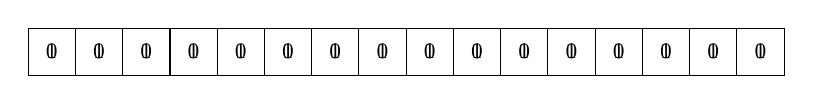
\begin{tikzpicture}
      \def\x{0.6}
      \foreach \i in {0,1,...,15}{
        \draw (-\i*\x,0)rectangle(-\i*\x-\x,\x);
        \ifthenelse{\i=1 \OR \i=3}
        {
          \node at (-\i*\x-0.5*\x,0.5*\x)[]{\footnotesize{1}};
        }
        {
          \node at (-\i*\x-0.5*\x,0.5*\x)[]{\footnotesize{0}};

        }
      }
    \end{tikzpicture}
    \caption{正数10的存储方式}
  \end{figure}
  % 
  \begin{figure}
    \centering
    \begin{tikzpicture}
      \def\x{0.6}
      \foreach \i in {0,1,...,15}{
        \draw (-\i*\x,0)rectangle(-\i*\x-\x,\x);
        \ifthenelse{\i=1 \OR \i=3}
        {
          \node at (-\i*\x-0.5*\x,0.5*\x)[]{\footnotesize{1}};
        }
        {
          \node at (-\i*\x-0.5*\x,0.5*\x)[]{\footnotesize{0}};
        }
      }
      \node at (-16*\x,1.3*\x) [right]{\footnotesize{10的原码}};
      %%%% 
      \foreach \i in {0,1,...,15}{
        \draw (-\i*\x,-2*\x)rectangle(-\i*\x-\x,-\x);
        \ifthenelse{\i=1 \OR \i=3}
        {
          \node at (-\i*\x-0.5*\x,-1.5*\x)[]{\footnotesize{0}};
        }
        {
          \node at (-\i*\x-0.5*\x,-1.5*\x)[]{\footnotesize{1}};
        }
      }
      \node at (-16*\x,-0.7*\x) [right]{\footnotesize{取反}};
      %%%% 
      \foreach \i in {0,1,...,15}{
        \draw (-\i*\x,-4*\x)rectangle(-\i*\x-\x,-3*\x);
        \ifthenelse{\i=0 \OR \i=3}
        {
          \node at (-\i*\x-0.5*\x,-3.5*\x)[]{\footnotesize{0}};
        }
        {
          \node at (-\i*\x-0.5*\x,-3.5*\x)[]{\footnotesize{1}};
        }
      }
      \node at (-16*\x,-2.7*\x) [right]{\footnotesize{加1,得-10的补码}};

    \end{tikzpicture}
    \caption{负数-10的存储方式}
  \end{figure}
\end{frame}

\begin{frame}[fragile]\ft{ \lst|int| 型}
  \lst|int| 型表示有符号整数,其取值范围依赖于系统。
  \begin{itemize}
  \item C:使用头文件 \lst|limits.h|
    \begin{itemize}
    \item 它专用于检测\red{整型数据类型}的取值范围。
    \end{itemize}
  \item C++:使用头文件 \lst|limits|
    \begin{itemize}
    \item 它提供了 \lst|std::numeric_limits| 模板类,用于替代C语言,检测\red{各种基本数据类型}的取值范围及其他信息。
    \end{itemize}
  \end{itemize}
\end{frame}
%
\begin{frame}[fragile]\ft{ \lst|int| 型}
  \lstinputlisting[basicstyle=\ttfamily\small]
  {slide03/code/int_info.c}
\pause 
\begin{lstlisting}[backgroundcolor=\color{red!10}]
$ gcc  int_info.c
$ ./a.out
range of int is -2147483648 ~ 2147483647
sizeof int = 4 bytes
\end{lstlisting}
\end{frame}

\begin{frame}[fragile]\ft{ \lst|int| 型}
  \lstinputlisting[basicstyle=\ttfamily\small]
  {slide03/code/int_info.cpp}
\pause 
\begin{lstlisting}[backgroundcolor=\color{red!10}]
$ g++  int_info.cpp
$ ./a.out
range of int is -2147483648 ~ 2147483647
sizeof int = 4 bytes
\end{lstlisting}
\end{frame}


\begin{frame}[fragile]\ft{ \lst|int| 变量的声明}
关键字 \lst|int| 用于声明基本的整型变量,书写格式为
\begin{lstlisting}[language=c,backgroundcolor=\color{red!10}]
int var;
int var1, var2;
\end{lstlisting}  \vspace{0.05in}

要声明多个变量,\vspace{0.05in}
\begin{itemize}
\item 可以逐个声明每个变量;\\[0.1in]
\item 也可在 \lst|int| 后跟一个变量名列表,各个变量之间用逗号隔开。
\end{itemize}

\end{frame}
% %
\begin{frame}[fragile]\ft{ \lst|int| 变量的赋值}
 \lst|int| 变量的赋值有如下三种方式:\vspace{0.05in}
\begin{enumerate}
\item 先声明,后赋值
\begin{lstlisting}
int n;
n = 1;
\end{lstlisting}
\item 先声明,后通过scanf函数赋值
\begin{lstlisting}
int n;
scanf("%d", &n);
\end{lstlisting} 
\item 初始化变量
\begin{lstlisting}
int n = 1;
\end{lstlisting} 
\end{enumerate}
\end{frame}
%
%
\begin{frame}[fragile]\ft{ \lst|int| 变量的初始化}
初始化变量就是为变量赋一个初始值。
\begin{lstlisting}[language=c,backgroundcolor=\color{red!10}]
int a = 1;
int b = 2, c = 3;
int d, e = 4;  // valid, but not good
\end{lstlisting}
请避免在一个声明语句中同时出现初始化和未初始化的变量。
\end{frame}
%
\begin{frame}[fragile]\ft{ \lst|int| 变量的初始化}
声明语句为变量创建、标定存储空间并为其指定初始值。 \pause 

\begin{figure}
\centering
\begin{tikzpicture}
\def\x{1}
\def\d{0}
\draw[thick,fill=gray!20] (0,\d)rectangle(5*\x,\d+0.5*\x);
\draw(2*\x,\d+0)--(2*\x,\d+0.5*\x);
\draw(3*\x,\d+0)--(3*\x,\d+0.5*\x);
\node at (2.5*\x,\d) [below] {b}; 
\node at (2.5*\x,\d+0.25*\x) [] {2}; 
\coordinate (b) at (-4*\x,\d);
\node at (b)  [above]{ \lst|int|  b=2;};
\draw[thick,->,>=stealth] (b) -- ++(0,-\x) -- 
node[above]{\footnotesize{分配存储空间并赋值}}
++(6.5*\x,0) -- ++(0,0.5*\x);

\def\d{2*\x}
\draw[thick,fill=gray!20] (0,\d)rectangle(5*\x,\d+0.5*\x);
\draw(2*\x,\d+0)--(2*\x,\d+0.5*\x);
\draw(3*\x,\d+0)--(3*\x,\d+0.5*\x);
\node at (2.5*\x,\d) [below] {a}; 
\coordinate (a) at (-4*\x,\d);
\node at (a)  [above]{ \lst|int|  a;};
\draw[thick,->,>=stealth] (a) -- ++(0,-\x) -- 
node[above]{\footnotesize{分配存储空间}}
++(6.5*\x,0) -- ++(0,0.5*\x);
\end{tikzpicture}
\caption{定义和初始化变量}
\end{figure}


\end{frame}
%
%
\begin{frame}[fragile]\ft{ \lst|int| 值的打印}
  \lstinputlisting[basicstyle=\ttfamily\small]
  {slide03/code/print1.c} 
\pause 

\begin{lstlisting}[backgroundcolor=\color{red!10}]
$ gcc print1.c
$ ./a.out
Doing it right: 10 - 2 = 8
Doing it wrong: 10 - 73832 = 771
\end{lstlisting}
\end{frame}
%
%
\begin{frame}[fragile]\ft{ \lst|int| 值的打印}

 第二次调用 \lst|print()| 时,程序使用 \lst|a| 为第一个 \lst|%d| 提供打印值,然后用内存中的任意值为其余两个 \lst|%d| 提供打印值。\vspace{0.1in}

 \begin{free}[注意]{}
   使用 \lst|printf()| 时,格式说明符的个数与要显示值的数目必须相同。
 \end{free}

 
\end{frame}
% %
% %
\begin{frame}[fragile]\ft{八进制数和十六进制数的打印}
在C中,有专门的前缀指明进制。

\begin{itemize}
\item 前缀 \lst|0x| 或 \lst|0X| 表示十六进制数\\[0.1in]
  \begin{itemize}
  \item \lst|16| 的十六进制表示为 \lst|0x10| 或 \lst|0X10|。\\[0.2in]
  \end{itemize}
\item 前缀 \lst|0| 表示八进制数\\[0.1in]
  \begin{itemize}
  \item \lst|16| 的八进制表示为 \lst|020|。
  \end{itemize}
\end{itemize}
\end{frame}

\begin{frame}[fragile]\ft{打印八进制数和十六进制数}
\lstinputlisting[language=c,frame=single,numbers=left]{
slide03/code/bases.c
}
% \end{frame}
% %
% %
% \begin{frame}[fragile]\ft{八进制数和十六进制数的打印}
\pause 
\begin{lstlisting}[language=c,backgroundcolor=\color{red!10}]
$ gcc bases.c
$ ./a.out
dec = 100; oct = 144; hex = 64
dec = 100; oct = 0144; hex = 0x64
\end{lstlisting}
\end{frame}
%
\begin{frame}[fragile]\ft{八进制数和十六进制数的打印}
\begin{table}
\centering
\begin{tabular}{p{2cm}|p{2cm}|p{4cm}} \hline
进制&格式说明符&格式说明符(显示前缀)\\\hline
十进制& \lst|%d| & \\
八进制& \lst|%o| & \lst|%#o|\\
十六进制& \lst|%x| 或 \lst|%X|  & \lst|%#x| 或 \lst|%#X|\\\hline
\end{tabular}
\end{table}
\end{frame}
% %
\begin{frame}[fragile]\ft{其他整数类型}
C/C++提供4个附属关键字修饰 \lst|int| :\lst|short|、\lst|long|、\lst|unsigned| 和 \lst|signed|。

\begin{table}
\centering
\begin{tabular}{p{4.5cm}|p{3cm}|p{2.8cm}} \hline
类型&含义&占位符\\\hline
\lst|short (int)|&   适用于小数值 &  \lst|%hd, %ho, %hx|\\[0.1in]\hline
\lst|long (int)| &   适用于大数值 &  \lst|%ld, %lo, %lx|\\[0.1in]\hline
\lst|long long (int)|& 适用于更大数值&  \lst|%lld, %llo, %llx|  \\
\hline
\lst|unsigned (int)|&    & \lst|%u|\\[0.1in]\hline
\lst|unsigned long (int)| &   & \lst|%lu| \\[0.1in]\hline
\lst|unsigned long long (int)|   &  &\lst|%llu|\\
\hline
\end{tabular}
\end{table}
\pause

关键字signed可以和任何有符号类型一起使用,使数据类型更加明确。
如short、short int、signed short和signed short int表示同一种类型。
\end{frame}
% %
\begin{frame}[fragile]\ft{其他数据类型}
  \begin{question}[]{}
    为什么会出现多种整数类型?
  \end{question}
  \pause 
  %C仅保证short类型不会比 \lst|int| 类型长,long类型不会比 \lst|int| 类型短,其目的是为了适应不同的机器。\vspace{0.05in}

  \begin{itemize}
  \item 有些CPU的自然字大小,若认为没有表示更大数的需要,会将long类型和 \lst|int| 类型定义相同的长度。\\[0.1in]
  \item 很多场合不要用到太大的整数,于是创建了更节省空间的short类型。
  \end{itemize}
\end{frame}

\begin{frame}[fragile]\ft{整数的上溢}
\begin{question}[]{}
若整数太大,超出整数类型的范围会发生什么?
\end{question}
\end{frame}

\begin{frame}[fragile]\ft{整数的上溢}
\lstinputlisting[language=c,frame=single,numbers=left]{
slide03/code/intOverflow.c
}
\end{frame}
%
\begin{frame}[fragile]\ft{整数的上溢}

\begin{lstlisting}[language=c,backgroundcolor=\color{red!10}]
$ gcc intOverflow.c
$ ./a.out
i = 2147483647, i+1 = -2147483648, i+2 = -2147483647
j = 4294967295, j+1 = 0, j+2 = 1
\end{lstlisting}
\end{frame}
%
\begin{frame}[fragile]\ft{整数的上溢}

当达到最大值时,将溢出到起始点。\vspace{0.05in}
\begin{itemize}
\item 对于unsigned int类型,起始点是0;\\[0.1in]
\item 对于int类型,起始点为-2147483648。
\end{itemize}

\vspace{0.1in}
 注意: 当整数溢出时,编译器不会给出任何提示,故编程时必须谨慎对待此类问题。 

\end{frame}

% \section{递归}

\begin{frame}[fragile]\ft{\secname}
C允许一个函数调用其自身,这种调用过程被称为递归(recursion)。 
\vspace{0.1in}

\begin{itemize}
\item 递归一般可用循环代替。有些情况使用循环会比较好,而有时使用递归更有效。\\[0.1in]
\item 递归虽然可使程序结构优美,但其执行效率却没循环语句高。
\end{itemize}
\end{frame}


\begin{frame}[fragile,allowframebreaks]\ft{\secname}
  \lstinputlisting
  [language=c,numbers=left,frame=single]
  {Code/recur.c}
\end{frame}


\begin{frame}[fragile]\ft{\secname}
\begin{lstlisting}[backgroundcolor=\color{red!10}]
Level 1: n location 0x7fff5fbff7bc
Level 2: n location 0x7fff5fbff79c
Level 3: n location 0x7fff5fbff77c
Level 4: n location 0x7fff5fbff75c
LEVEL 4: n location 0x7fff5fbff75c
LEVEL 3: n location 0x7fff5fbff77c
LEVEL 2: n location 0x7fff5fbff79c
LEVEL 1: n location 0x7fff5fbff7bc
\end{lstlisting}
\end{frame}


\begin{frame}[fragile]\ft{\secname}
{\tf \&}为地址运算符,{\tf \&n}表示存储n的内存地址,{\tf printf()}使用占位符{\tf \%p}来指示地址。
\end{frame}


\begin{frame}[fragile]\ft{\secname:程序分析}
\begin{itemize}
\item 首先,{\tf main()}使用实参1调用{\tf up\_and\_down()},打印语句{\tf \#1}输出{\tf Level 1}。\\[0.1in]
\item 然后,由于$n<4$,故{\tf up\_and\_down()}(第1级)使用实参2调用{\tf up\_and\_down()}(第2级),打印语句{\tf \#1}输出{\tf Level 2}。\\[0.1in]
\item 类似地,下面的两次调用打印{\tf Level 3}和{\tf Level 4}。
\end{itemize}
\end{frame}

\begin{frame}[fragile]\ft{\secname:程序分析}
\begin{itemize}
\item 当开始执行第4级调用时,$n$的值为4,故if语句不满足条件,不再继续调用{\tf up\_and\_down()},接着执行打印语句{\tf \#2},输出{\tf Level 4},至此第4级调用结束,把控制返回给第3级调用函数。\\[0.1in]
\item 第3级调用函数中前一个执行过的语句是在if语句中执行第4级调用,因此,它开始执行后续代码,即执行打印语句{\tf \#2},输出{\tf Level 3}。\\[0.1in]
\item 当第3级调用结束后,第2级调用函数开始继续执行,输出{\tf Level 2}。以此类推。
\end{itemize}
\end{frame}

\begin{frame}[fragile]\ft{\secname:递归的基本原理}
\begin{itemize}
\item
\textcolor{acolor1}{每一级的递归都使用其私有变量n。}\\[0.1in]
\item
每一次函数调用都会有一次返回。当程序执行到某一级递归的结尾处时,它会转移到前一级递归继续执行。
\end{itemize}
\end{frame}

\begin{frame}[fragile]\ft{\secname:递归的基本原理}
\begin{itemize}
\item
递归函数中,位于递归调用前的语句和各级被调函数具有相同的执行次序。\\[0.1in]
\item[] 如打印语句\#1位于递归调用语句之前,它按递归调用的顺序执行4次,即依次为第1级、第2级、第3级和第4级。\\[0.1in]
\item 
递归函数中,位于递归调用后的语句和各级被调函数具有相反的执行次序。\\[0.1in]
\item[] 
如打印语句{\tf \#2}位于递归调用语句之后,执行次序为:第4级、第3级、第2级和第1级。
\end{itemize}
\end{frame}

\begin{frame}[fragile]\ft{\secname:递归的基本原理}
\begin{itemize}
\item 递归函数中,必须包含可以终止递归调用的语句。
\end{itemize}

\end{frame}

\begin{frame}[fragile]\ft{\secname:尾递归}
最简单的递归方式是\textcolor{acolor1}{把递归调用语句放在函数结尾,return语句之前。}这种形式被称为\textcolor{acolor1}{尾递归(tail recursion)}。尾递归的作用相当于一条循环语句,它是最简单的递归形式。
\end{frame}

\begin{frame}[fragile]\ft{\secname:尾递归}
分别使用循环和尾递归编写函数计算阶乘,然后用一个驱动程序测试它们。
\end{frame}

\begin{frame}[fragile,allowframebreaks]\ft{\secname:尾递归}
  \lstinputlisting
  [language=c,numbers=left,frame=single]
  {Code/factor.c}
\end{frame}


\begin{frame}[fragile]\ft{\secname:尾递归}
\begin{lstlisting}
This program calculates factorials.
Enter a value in the range 0-12 (q to quit):
5
loop:      5! = 120
recursion: 5! = 120
Enter a value in the range 0-12 (q to quit):
10
loop:      10! = 3628800
recursion: 10! = 3628800
Enter a value in the range 0-12 (q to quit):
12
loop:      12! = 479001600
recursion: 12! = 479001600
Enter a value in the range 0-12 (q to quit):
q
Bye.
\end{lstlisting}
\end{frame}

\begin{frame}[fragile]\ft{\secname:尾递归}
{\Large 选用循环还是递归?}\pause 一般来说,选择循环更好一些。
\pause
\vspace{0.1in}

\begin{itemize}
\item 每次递归调用都有自己的变量集合,需要占用较多的内存。每次递归调用需要把新的变量集合存储在堆栈中。\\[0.1in]
\item 每次函数调用都要花费一定的时间,故递归的执行速度较慢。
\end{itemize}
\end{frame}

\begin{frame}[fragile]\ft{\secname:尾递归}
{\Large 那为什么要学习递归呢?}\pause 
\vspace{0.1in}

\begin{itemize}
\item 尾递归非常简单,易于理解。\\[0.1in]
\item 某些情况下,不能使用简单的循环语句代替递归,所以有必要学习递归。
\end{itemize}

\end{frame}

\begin{frame}[fragile]\ft{\secname:递归与反向计算}
编写程序,将一个整数转换为二进制形式。
\end{frame}

\begin{frame}[fragile]\ft{\secname:递归与反向计算}
对于奇数,其二进制形式的末位为1;而对于偶数,其二进制形式的末位为0。于是,\textcolor{acolor1}{对于n,其二进制数的末位为n\%2。}
\begin{lstlisting}[backgroundcolor=\color{red!10}]
628
628%10=8  628/10=62  62%10=2   62/10=6   6%10=6
     8                     2                  6
\end{lstlisting}

\begin{lstlisting}[backgroundcolor=\color{red!10}]
5  
 5%2=1  5/2=2  2%2=0  2/2=1  1%2=1
     1             0             1 
10
10%2=0  10/2=5  5%2=1  5/2=2  2%2=0  
     0              1             0
2/2=1  1%2=1
           1
\end{lstlisting}

\end{frame}

\begin{frame}[fragile]\ft{\secname:递归与反向计算}
规律:
\vspace{0.1in}

\begin{itemize}
\item 
在递归调用之前,计算{\tf n\%2}的值,在递归调用之后输出。\\[0.1in]
\item
为算下一个数字,需把原数值除以2。若此时得出的为偶数,则下一个二进制位为0;若得出的是奇数,则下一个二进制位为1。
\end{itemize}
\end{frame}

\begin{frame}[fragile,allowframebreaks]\ft{\secname:递归与反向计算}
\lstinputlisting
  [language=c,numbers=left,frame=single]
  {Code/binary.c}
\end{frame}



\begin{frame}[fragile]\ft{\secname:递归与反向计算}
\begin{lstlisting}[backgroundcolor=\color{red!10}]
Enter an integer (q to quit):
9
Binary equivalent: 1001
Enter an integer (q to quit):
255
Binary equivalent: 11111111
Enter an integer (q to quit):
1024
Binary equivalent: 10000000000
Enter an integer (q to quit):
q
Done.
\end{lstlisting}
\end{frame}


\begin{frame}[fragile]\ft{\secname:递归的优缺点}
 

\begin{itemize}
\item 优点:
\item[] 
为某些编程问题提供了最简单的解决办法。\\[0.1in]
\item 缺点:
\item[]
一些递归算法会很快地耗尽计算机的内存资源,同时递归程序难于阅读和维护。
\end{itemize}

\end{frame}


\begin{frame}[fragile]\ft{\secname:递归的优缺点}
编写程序,计算斐波那契数列。
$$
\begin{aligned}
&F_1=F_2=1,\\[0.1in]
&F_n=F_{n-1}+F_{n-2}, \quad n=3,4,\cd.
\end{aligned}
$$
\end{frame}


\begin{frame}[fragile]\ft{\secname:递归的优缺点}
\begin{lstlisting}
long Fibonacci(int n)
{
  if (n > 2)
    return Fibonacci(n-1) + Fibonacci(n-2);
  else
    return 1;
}
\end{lstlisting}

该函数使用了双重递归(double recursion),即函数对本身进行了两次调用。这会导致一个弱点。{\Huge What?}
\end{frame}


\begin{frame}[fragile]\ft{\secname:递归的优缺点}
每级调用的变量数会呈指数级增长:
\begin{table}
\centering
\caption{每级调用中变量n的个数}
\begin{tabular}{cc}\hline
Level & number of n\\\hline
$1$ & $1$\\
$2$ & $2$\\
$3$ & $2^2$\\
$4$ & $2^3$\\
$\vd$ & $\vd$ \\
$l$ & $2^{l-1}$\\\hline
\end{tabular}
\end{table}
\end{frame}

% \subsection{重定向与文件}



\begin{frame}[fragile]\ft{\subsecname}
\end{frame}
% \section{创建一个更友好的用户界面}
\begin{frame}[fragile]\ft{\secname}
  \begin{free}[例]{}
    编制一个猜字程序,看是否为1-100之间的某个整数。程序会依次问你是否为1、2、3、$\cd$,你回答 \lstinline|y| 表示 \lstinline|yes|,回答 \lstinline|n| 表示 \lstinline|no|,直到回答正确为止。
  \end{free}
\end{frame}


\begin{frame}[fragile,allowframebreaks]\ft{\secname}
  \lstinputlisting
  [basicstyle=\ttfamily\small]
  {slide08/code/guess.c}
\end{frame}

\begin{frame}[fragile]\ft{\secname}
\begin{lstlisting}[backgroundcolor=\color{blue!20}]
Pick an integer from 1 to 100. I will try to guess it.
Respond with a y if my guess is right and with
an n if it is wrong.
Uh...is your number 1?
n
Well, then, is it 2?
Well, then, is it 3?
n
Well, then, is it 4?
Well, then, is it 5?
y
I knew I could do it!
\end{lstlisting}
\end{frame}

\begin{frame}[fragile]\ft{\secname}
输入 \lstinline|n| 时,竟然做了两次猜测,Why? \pause \vspace{0.1in}

\red{换行符在作怪!}
\pause \vspace{0.1in}

\begin{itemize}
\item 读入字符 \lstinline|'n'|,因 \lstinline|'n' != 'y'|,故打印
\begin{lstlisting}
Well, then, is it 2?
\end{lstlisting}
\item 紧接着读入字符 \lstinline|'\n'|,因 \lstinline|'\n' != 'y'|,故打印
\begin{lstlisting}
Well, then, is it 3?
\end{lstlisting}
\end{itemize}
\end{frame}

\begin{frame}[fragile]\ft{\secname:解决方案}
使用一个 \lstinline|while| 循环来丢弃输入行的其它部分,包括换行符。
\begin{lstlisting}[]
while (getchar() != 'y')
{
  printf("Well, then, is it %d?\n", ++guess);
  while (getchar() != '\n')
    continue;  // skip rest of input line
}
\end{lstlisting}
这种处理办法还能把诸如 \lstinline|no| 和 \lstinline|no way| 这样的输入同简单的n一样看待。
\end{frame}

\begin{frame}[fragile]\ft{\secname}
\begin{lstlisting}
Pick an integer from 1 to 100. I will try to guess it.
Respond with a y if my guess is right and with
an n if it is wrong.
Uh...is your number 1?
n
Well, then, is it 2?
no
Well, then, is it 3?
no sir
Well, then, is it 4?
forget it
Well, then, is it 5?
y
I knew I could do it!
\end{lstlisting}
\end{frame}

% \begin{frame}[fragile]\ft{\secname}
% 若不希望将f的含义看做与n相同,可使用一个if语句来筛选掉其它响应。
% \begin{lstlisting}[language=c,numbers=left,frame=single]
% char ch;
% ...
% while ((ch = getchar()) != 'y')
% {
%   if (ch == 'n')
%     printf("Well, then, is it %d?\n", ++guess);
%   else
%     printf("Sorry, I understand only y or n.\n");
%   while (getchar() != '\n')
%     continue;  // skip rest of input line
% }
% \end{lstlisting}


% \end{frame}

% \begin{frame}[fragile]\ft{\secname}
% \begin{lstlisting}
% Pick an integer from 1 to 100. I will try to guess it.
% Respond with a y if my guess is right and with
% an n if it is wrong.
% Uh...is your number 1?
% n
% Well, then, is it 2?
% no
% Well, then, is it 3?
% no sir
% Well, then, is it 4?
% forget it
% Sorry, I understand only y or n.
% n
% Well, then, is it 5?
% y
% I knew I could do it!
% \end{lstlisting}

% \end{frame}

% \begin{frame}[fragile]\ft{\secname}
% 当你编写交互式程序时,应试着去预料用户未能遵循指示的可能方式,然后让程序能合理地处理用户的疏忽。并告诉用户哪里出了错误,给予他们另一次机会。
% \end{frame}

% \begin{frame}[fragile]\ft{\secname:混合输入数字和字符}
% 若你的程序需要使用{\tf getchar()}输入字符和使用{\tf scanf()}输入数字。两个函数都很很好的独立完成其工作,但不能很好的混合在一起。因为
% \begin{itemize}
% \item
% {\tf getchar()}读取每个字符,包括空格、制表符和换行符
% \item
% {\tf scanf()}在读取数字时会跳过空格、制表符和换行符。
% \end{itemize}
% \end{frame}

% \begin{frame}[fragile]\ft{\secname:混合输入数字和字符}
% 编写程序,读取一个字符和两个整数,然后使用这两个整数指定行数和列数打印该字符。
% \end{frame}

% \begin{frame}[fragile,allowframebreaks]\ft{\secname:混合输入数字和字符}
% \lstinputlisting
% [language=c,numbers=left,frame=single]
% {slide08/code/showchar1.c}
% \end{frame}

% \begin{frame}[fragile]\ft{\secname:混合输入数字和字符}
% \begin{lstlisting}
% Enter a character and two integers:
% c 2 3[enter]
% ccc
% ccc
% Enter another character and two integers;
% Enter a newline to quit.
% Bye.
% \end{lstlisting}
% \end{frame}

% \begin{frame}[fragile]\ft{\secname:混合输入数字和字符}
% \begin{itemize}
% \item
% 程序开始时表现很好。当你输入c 2 3时,如期打印2行3列c字符。\\[0.1in]
% \item
% 然后程序提示输入第二组数据,但还没等你输入程序就退出了。Why? \pause \\[0.1in]
% \item[] 又是它在作怪!\pause 谁?\pause 换行符! \pause \\[0.1in]
% \item 
% 输入第一组数据后按下了换行符,scanf将它留在了输入队列。
% \\[0.1in]
% \item[] 而{\tf getchar()}并不跳过换行符,故在下一次循环时,{\tf getchar()}读取了该字符,并将其值赋给了ch,而ch为换行符正是终止循环的条件。
% \end{itemize}
% \end{frame}

% \begin{frame}[fragile]\ft{\secname:解决方案}
% \begin{itemize}
% \item
% 程序必须跳过一个输入周期中最后一个数字与下一行开始出键入的字符之间的所有换行符或空格。 \\[0.1in]
% \item
% 若除了{\tf getchar()}判断之外还可以在{\tf scanf()}阶段终止程序,则会更好。
% \end{itemize}
% \end{frame}

% \begin{frame}[fragile,allowframebreaks]\ft{\secname:混合输入数字和字符}
% \lstinputlisting
% [language=c,numbers=left,frame=single]
% {slide08/code/showchar2.c}
% \end{frame}
% \begin{frame}[fragile]\ft{\secname:混合输入数字和字符}
% \begin{lstlisting}[backgroundcolor=\color{blue!20}]
% Enter a character and two integers:
% c 1 3[enter]
% ccc
% Enter another character and two integers;
% Enter a newline to quit.
% ! 3 6[enter]
% !!!!!!
% !!!!!!
% !!!!!!
% Enter another character and two integers;
% Enter a newline to quit.

% Bye.
% \end{lstlisting}
% \end{frame}

% \section{关键字}
\begin{frame}[fragile]\ft{\secname}
关键字是C中的特殊词汇,不能用它们来对变量或者函数命名。
若试图把一个关键字作为变量名,编译器把它当做一个语法错误。
\end{frame}

\begin{frame}[fragile]\ft{\secname}
\begin{table}
\centering
%\caption{C关键字}
\begin{tabular}{p{2cm}|p{2cm}|p{2cm}|p{2cm}}\hline
auto & enum & restrict & unsigned \\
break & extern & return & void \\
case & float & short & volatile \\
char & for & signed & while \\
const & goto & sizeof & \_Bool \\
continue & if & static & \_Complex \\
default & inline & struct & \_Imaginary\\
do & int & switch &  \\
double & long & typedef & \\
else & register & union \\ \hline
\end{tabular}
\end{table}
\end{frame}










\section{编译C程序的工作原理}
\begin{frame}\ft{\secname}
  C是一种高级语言,它需要编译器将其转换为可执行代码,以使得程序能在机器上运行。 

  以下介绍在MAC或Linux上使用gcc编译器的几个步骤。

\end{frame}


\begin{frame}[fragile]\ft{\secname}
  \begin{itemize}

  \item[(1)] 首先使用编辑器(如vi或emacs等)创建一个C程序,并将其保存为hello.c。

    \begin{lstlisting}
$ emacs hello.c
    \end{lstlisting}
  \end{itemize}
\end{frame}

\begin{frame}[fragile]\ft{\secname}
  \begin{itemize}
  \item[] 
    在编辑界面输入以下内容:
    \lstinputlisting[]{slide01/code/hello.c}

  \end{itemize}
\end{frame}

\begin{frame}[fragile]\ft{\secname}
  \begin{itemize}
  \item[(2)] 然后用以下命令编译,并查看当前目录下的文件。
    \begin{lstlisting}[backgroundcolor=\color{red!10}]
$ gcc -Wall hello.c –o hello
$ ls
  hello    hello.c
\end{lstlisting}

\begin{itemize}
\item 选项 \blue{\lstinline|-Wall|} 启动所有编译器的警告信息。建议使用该选项以生成更好的代码。
\item 选项 \blue{\lstinline|-o|} 用来制定输出文件名。如果缺省该选项,则输出文件将默认为 \blue{\lstinline|a.out|}。
\end{itemize}
    
  \end{itemize}
\end{frame}

\begin{frame}[fragile]\ft{\secname}
  \begin{itemize}
  \item[(3)] 编译通过后,将会生成可执行文件。可用以下命令来运行:
    \begin{lstlisting}[backgroundcolor=\color{red!10}]
$ ./hello
Hello World!
    \end{lstlisting}
  \end{itemize}
\end{frame}



\begin{frame}[fragile]\ft{\secname}
  \href{https://blog.csdn.net/elfprincexu/article/details/45043971}{编译器将一个C程序转换为一个可执行文件},需经历了4个阶段:
  \begin{itemize}
  \item 预处理
  \item 编译
  \item 汇编
  \item 链接
  \end{itemize}

  \begin{figure}
    \centering
    \includegraphics[width=4in]{slide01/images/compile.png}
    \caption{编译过程}
    \label{fig:1}
  \end{figure}
  
\end{frame}


\begin{frame}[fragile]\ft{\secname}
  执行以下命令,会在当前目录下生成所有的中间文件以及可执行文件。
  \begin{lstlisting}[backgroundcolor=\color{red!10}]
    $ gcc -Wall -save-temps hello.c –o hello 
    $ ls 
    hello     hello.c   hello.o
    hello.i   hello.s
  \end{lstlisting}
\end{frame}


\begin{frame}[fragile]\ft{\secname} 
  \begin{itemize}
  \item[(1)] \red{预处理阶段}
\begin{lstlisting}[backgroundcolor=\color{red!10}]
$ gcc -E hello.c –o hello.i 
\end{lstlisting}    
\end{itemize}

在该阶段,
    \begin{itemize}
    \item 去掉注释
    \item 宏的展开
    \item 头文件的展开
    \item 选项 \blue{\lstinline|-E|} 的作用是让gcc在预处理结束后停止编译过程。
    \end{itemize}   
\end{frame}


\begin{frame}[fragile]\ft{\secname}
  \begin{lstlisting}[basicstyle=\ttfamily\footnotesize,backgroundcolor=\color{red!10}]
    $ less hello.i
    $ ls 
    ...
    extern int printf (const char *__restrict __format, ...);
    ...
    # 868 "/usr/include/stdio.h" 3 4
    # 5 "hello.c" 2
    # 5 "hello.c"

    int main(void)
    {
      printf("Hello World!\n");
      return 0;
    }
  \end{lstlisting}
\end{frame}


% \begin{frame}[fragile]\ft{\secname}
%   \blue{分析:}在以上内容中,源文件被附加了很多信息,但在末尾代码仍被保留。{\ttfamily printf()}函数中包含了{\ttfamily a+b}而非{\ttfamily add(a,b)},因为宏已被展开。注释被去除掉。{\ttfamily\#include<stdio.h>}没有了,取而代之的是很多代码。因此,头文件已被展开,并且被包含到了源文件中。

% \end{frame}


\begin{frame}[fragile]\ft{\secname}
  \begin{itemize}
  \item[(2)] 编译阶段
\begin{lstlisting}[backgroundcolor=\color{red!10}]
$ gcc -S hello.i –o hello.s
\end{lstlisting}
\end{itemize}

在该阶段,
\begin{itemize}
\item 检查代码的规范性、是否有语法错误等
\item 检查无误后,将代码翻译成汇编语言
\item 选项 \blue{\lstinline|-S|} 只进行编译,不进行汇编,生成汇编代码。 
\end{itemize}

\end{frame}


\begin{frame}[fragile]\ft{\secname}
  \begin{lstlisting}[basicstyle=\ttfamily\footnotesize,backgroundcolor=\color{red!10}]
    $ less hello.s
    ...
    movl    $0, -4(%rbp)
    movl    $5, -8(%rbp)
    movl    $4, -12(%rbp)
    movl    -8(%rbp), %eax
    addl    -12(%rbp), %eax
    movl    %eax, %esi
    movb    $0, %al
    callq   _printf
    xorl    %esi, %esi
    ...      
  \end{lstlisting}
  % 以上内容表明这是汇编语言,能为汇编器所识别。
\end{frame}


\begin{frame}[fragile]\ft{\secname}
  \begin{itemize}
  \item[(3 )] 汇编阶段
\begin{lstlisting}[backgroundcolor=\color{red!10}]
$ gcc -c hello.s –o hello.o
\end{lstlisting}   
\end{itemize}

在该阶段,
\begin{itemize}
\item 将通过汇编器将 \lstinline|hello.s| 转换成  二进制机器指令文件\lstinline|hello.o|。
\item 只会将现有代码转换成机器语言,而诸如 \lstinline|printf()| 的函数调用则不会。
\item 选项 \blue{\lstinline|-c|} 的作用是将汇编代码转换为二进制目标代码。
\end{itemize}
\end{frame}


\begin{frame}[fragile]\ft{\secname}
  \begin{lstlisting}[backgroundcolor=\color{red!10}]
    $ less hello.o
    <CF><FA><ED><FE>^G^@^@^A^C^@^@^@^A^@^@^@^D^@^@^@^@^B^@^@^@ ^@^@^@^@^@^@^Y^@^@^@<88>^A^@^@^@^@^@^@^@^
    ...      
  \end{lstlisting}

\end{frame}


\begin{frame}[fragile]\ft{\secname}
  \begin{itemize}
  \item[(4)] 链接阶段
  \item[] 
    这里涉及一个重要的概念:\red{函数库}。 
  \end{itemize} \pause
  \begin{question}[]{}
    在 \lstinline|hello.c|中,并没有定义 \blue{\lstinline|printf()|} 的函数实现,并且在 \blue{\lstinline|stdio.h|} 也只有函数的声明,没有定义函数的实现。那么,是在哪里实现了 \blue{\lstinline|printf()|} 呢?
  \end{question} \pause

  事实上,系统将这些函数的定义编译后放在了相应的函数库中。在没有特别指定时,gcc 会到系统默认的搜索路径 \blue{\lstinline|/usr/lib|} 下进行查找,连接到相关的库函数后,就能使用 \blue{\lstinline|printf()|}了,而这就是链接的作用。
 
\end{frame}


% \begin{frame}[fragile]\ft{\secname}
%   在命令行中输入以下命令,可看出从目标文件到可执行文件时文件大小的变化。这是因为链接器为我们的程序添加了额外的代码。
%   \begin{lstlisting}[basicstyle=\ttfamily\footnotesize,backgroundcolor=\color{red!10}]
%     $ size hello.o
%     __TEXT  __DATA  __OBJC  others    dec         hex
%     145     0       0       32      177         b1        
%     $ size hello
%     __TEXT  __DATA  __OBJC  others    dec         hex
%     4096      4096    0  4294971392 4294979584 100003000
%   \end{lstlisting}

% \end{frame}


\begin{frame}{函数库}
  \href{http://www.cnblogs.com/skynet/p/3372855.html}{函数库}一般分为静态库和动态库。
  \begin{defn}[静态库]{}
    在链接阶段,将汇编生成的目标文件.o与引用到的库文件一起链接打包到可执行文件,对应的链接方式成为\red{静态链接}。
  \end{defn}

  \begin{defn}[动态库]{}
    \red{动态库}在程序编译时并不会被连接到目标代码中,而是在程序运行是才被载入。
  \end{defn}
\end{frame}

\begin{frame}{静态库}
  \begin{free}[静态库的特点]{}
    \begin{itemize}
    \item 一个静态库可以简单看成是一组目标文件(.o/.obj文件)的集合,即很多目标文件经过压缩打包后形成的一个文件。\\[.1in]
    \item 静态库对函数库的链接是放在编译时期完成的 \\[.1in]
    \item 程序在运行时与函数库再无瓜葛,移植方便 \\[.1in]
    \item 浪费空间与资源,因为所有相关的目标文件与牵涉到的函数库被链接合并成一个可执行文件\\[.1in]
    \item 后缀名为 \blue{\lstinline|.a|} (linux) 或 \blue{\lstinline|.lib|} (windows)
    \end{itemize}
  \end{free}

\end{frame}

\begin{frame}{静态库}
  \begin{figure}
    \centering
    \includegraphics[width=3.5in]{slide01/images/lib.png}
    % \caption{静态库}
  \end{figure}
\end{frame}

\begin{frame}{静态库}
  \begin{free}[静态库的缺点]{}
    \begin{itemize}
    \item 空间浪费
    \item 静态库对程序的更新、部署和发布页会带来麻烦。如果静态库liba.lib更新了,所以使用它的应用程序都需要重新编译、发布给用户(对于玩家来说,可能是一个很小的改动,却导致整个程序重新下载,全量更新)。    
    \end{itemize}
  \end{free}
\end{frame}


\begin{frame}{动态库}
  \begin{free}[动态库的特点]{}
    \begin{itemize}
    \item 不同的应用程序如果调用相同的库,那么在内存里只需要有一份该共享库的实例,规避了空间浪费问题。 \\[.05in]
    \item 动态库在程序运行是才被载入,也解决了静态库对程序的更新、部署和发布页会带来麻烦。用户只需要更新动态库即可,增量更新。 \\[.05in]
    \item 后缀名为 \blue{\lstinline|.so|} (linux) 或 \blue{\lstinline|.dll|} (windows) \\[0.05in]
    \item gcc 在编译时默认使用动态库
    \end{itemize}
  \end{free}

\end{frame}


\begin{frame}{动态库}
  \begin{figure}
    \centering
    \includegraphics[width=3.5in]{slide01/images/dll.png}
    %\caption{动态库}
  \end{figure}
\end{frame}

\begin{frame}{函数库的创建与使用}
  设有4个文件:
  \begin{itemize}
  \item \lstinline|hello.h|
  \item \lstinline|hello1.c|
  \item \lstinline|hello2.c|
  \item \lstinline|main.c|
  \end{itemize}
  我们来看看如何创建静态库与动态库,并如何使用它们。
\end{frame}

\begin{frame}{函数库的创建与使用}
  \lstinputlisting[title=hello.h]{slide01/code/lib/hello.h}
\end{frame}

\begin{frame}{函数库的创建与使用}
  \lstinputlisting[title=hello1.c]{slide01/code/lib/hello1.c}

  \lstinputlisting[title=hello2.c]{slide01/code/lib/hello2.c}
\end{frame}

\begin{frame}{函数库的创建与使用}
  \lstinputlisting[title=main.c]{slide01/code/lib/main.c}
\end{frame}

\begin{frame}[fragile]{静态库的创建与使用}

  \begin{lstlisting}
# 将 hello.c 编译成 hello.o (静态库和动态库都由 .o 文件生成)
$ gcc -c hello1.c hello2.c

# 为遵循 linux 中静态库的命名规范,静态库命名为 libhello.a
$ ar -crv libhello.a hello1.o hello2.o

# 将 main.c 与静态库连接,生成可执行文件 main
$ gcc main.c -L. -lhello -o main

# 运行 main
$ ./main
  \end{lstlisting}
  
\end{frame}


\begin{frame}[fragile]{动态库的创建与使用}

  \begin{lstlisting}
# 将 hello.c 编译成一个动态库 libhello.so
$ gcc hello1.c hello2.c -fPIC -shared -o libhello.so

# 将 main.c 与动态库连接,生成可执行文件 main
$ gcc main.c -L. -lhello -o main 

# 运行 main
$ ./main
  \end{lstlisting}
  
\end{frame}




\end{document}
